\documentclass[border=0mm,svgnames,export]{standalone}
\usepackage{pgfplots,amsmath}
\usepackage{animate} 

\begin{document}
\begin{animateinline}[palindrome,controls]{12} 
    \multiframe{1}{i=0+1}{% 
    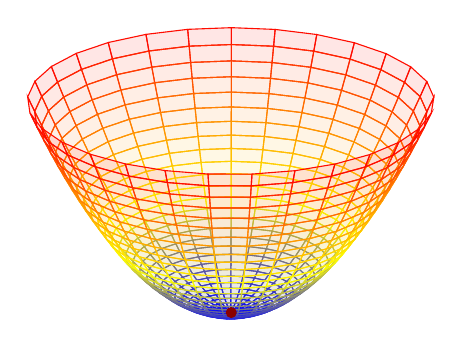
\begin{tikzpicture}
        \begin{axis}[
            hide axis,
            %axis lines=middle,
%            axis on top,
%            axis line style={blue,dashed,thick},
%            ymin=-2,ymax=2,
%            xmin=-2,xmax=2,
%            zmin=-2,zmax=2,
            samples=30,
            domain=0:360,
        ]
        \addplot3 [surf,shader=flat, z buffer=sort,fill opacity=0.1]
           ({sin(x)*y}, {cos(x)*y}, {(y^2-1)});
        % \draw[blue,thick,dashed] (axis cs:0,0,0) -- (axis cs:1,0,0)
        %             node[below,font=\footnotesize]{$\phi_{\text{IM}}$};
        % \draw[blue,thick,-stealth] (axis cs:1,0,0) -- (axis cs:1.3,0,0)
        %             node[above,font=\footnotesize]{$\hat{y}$};
        % \draw[blue,thick,dashed] (axis cs:0,0,0) -- (axis cs:0,-1,0)
        %             node[left=2mm,font=\footnotesize]{$\phi_{\text{RE}}$};
        % \draw[blue,thick,-stealth] (axis cs:0,-1,0) -- (axis cs:0,-1.5,0)
        %             node[right=1mm,font=\footnotesize]{$\hat{x}$};
        % \draw[blue,thick,dashed] (axis cs:0,0,0) -- (axis cs:0,0,1)
        %             %node[left=2mm,font=\footnotesize]{$\phi_{\text{RE}}$}
        %             ;
        % \draw[blue,thick,-stealth] (axis cs:0,0,1) -- (axis cs:0,0,1.3)
        %             node[right,font=\footnotesize]{$\hat{z}$};
        \coordinate (ca) at ({cos(3)},{sin(3)},0);
            \fill[DarkRed] (ca) circle (2pt);
        % \else
        % \ifnum\i<6
        % \pgfmathsetmacro\result{\i*5}
        %     \coordinate (ca) at (axis cs:{cos(\result)},{sin(\result)},0);
        %     \fill[DarkRed] (ca) circle (2pt);
        % % \else
        % %     \coordinate (ca) at (axis cs:{cos(30-\ang)},{sin(30-\ang)},0);
        % %     \fill[DarkRed] (ca) circle (2pt);
        % \fi
        \end{axis}
    \end{tikzpicture}
    }
\end{animateinline}
\end{document}